\section{データと計算の方法}
\label{sec:method}

\subsection{使ったデータ}

\begin{center}
\small
\resizebox{\linewidth}{!}{%
\begin{tabular}{lll}
\toprule
用途 & データ & 内容 \\
\midrule
上空の風 & JRA-3Q（気象庁の再解析） & \ang{0.375} 格子、1000--\SI{3}{\hecto\pascal} の 38 面、00 UTC \\
積雪・地上気象 & ERA5（ECMWF の再解析） & \ang{0.25} 格子。積雪深（12 時）、地上 \SI{10}{\metre} 風（9 時）、降水（9--12 時） \\
地上気象の確認 & アメダス（気象庁） & 芦辺（壱岐）・平戸・唐津の 9 時の観測 \\
地形 & NOAA NCEI の DEM & 約 \SI{600}{\metre} 間隔。平野・海岸からの距離 \\
市街地 & 国土数値情報 人口集中地区（2020 年） & 47 都道府県 \\
広場 & OpenStreetMap & 公園・グラウンドと、電線・建物の位置 \\
\bottomrule
\end{tabular}}
\end{center}

期間は 2016--2025 年の 12・1・2 月で、903 日ある（2016 年 1・2 月から 2025 年 12 月まで）。
シーズン単位（12 月〜翌 2 月）で数えるときは、12 月から 2 月までそろった 2016/17--2024/25 の
9 シーズンを使った。

\subsection{落下点の計算}

打ち上げ候補は、日本の陸地に \ang{0.05}（約 \SI{5}{\kilo\metre}）間隔で置いた
15{,}324 点である。朝鮮半島・中国・ロシア（北方領土を含む）は除いた。

各候補・各日について、その日 00 UTC（9 時 JST）の JRA-3Q の風の中で軌道を計算した。
上昇と降下のそれぞれで、気圧面ごとの層（隣の面との中点で区切る）を順に通り、
層の中では\textbf{その時点の位置で}風を双線形補間して進める。
風は打ち上げ時刻の解析値で固定している。降下速度は空気の密度に応じて変え、
上空ほど速く落ちる。

以前の研究では風を打ち上げ地点の 1 本の鉛直分布で固定していた。今回は位置に応じて
風を引き直すので、\SI{250}{\kilo\metre} 流される間の風の違いも入る。
壱岐のある 1 日で比べると、2 つの方法の落下点の差は約 \SI{3}{\kilo\metre} だった。

\subsection{飛行条件のばらつき}

同じ風でも、気球ごとに上昇速度や破裂高度は変わる。上位 16 地点については、
上昇速度（1 シグマで \SI{10}{\percent}）、破裂高度（\SI{1.5}{\kilo\metre}）、
降下速度（\SI{10}{\percent}）を正規分布で 64 通り振り、日ごとに 64 本のうち何本が
目標に落ちたかを、その日の成功の確率とした。本文の確率はすべてこの 64 本の平均である。

\subsection{確率の不確かさ}

同じ冬の中の日どうしは天気が続くので、903 日を独立な標本として扱うと区間が狭く出すぎる。
そこで 2016--2025 年の 10 年を年ごとに復元抽出するブロック・ブートストラップ（4000 回）で
95\% 区間を出した。この区間は「10 年の中で年による違いがどれだけあるか」を表しており、
データや判定基準の誤差は含まない。それらは \ref{sec:sensitivity} 節と \ref{sec:limits} 節で扱う。

\begin{figure}[htbp]
\centering
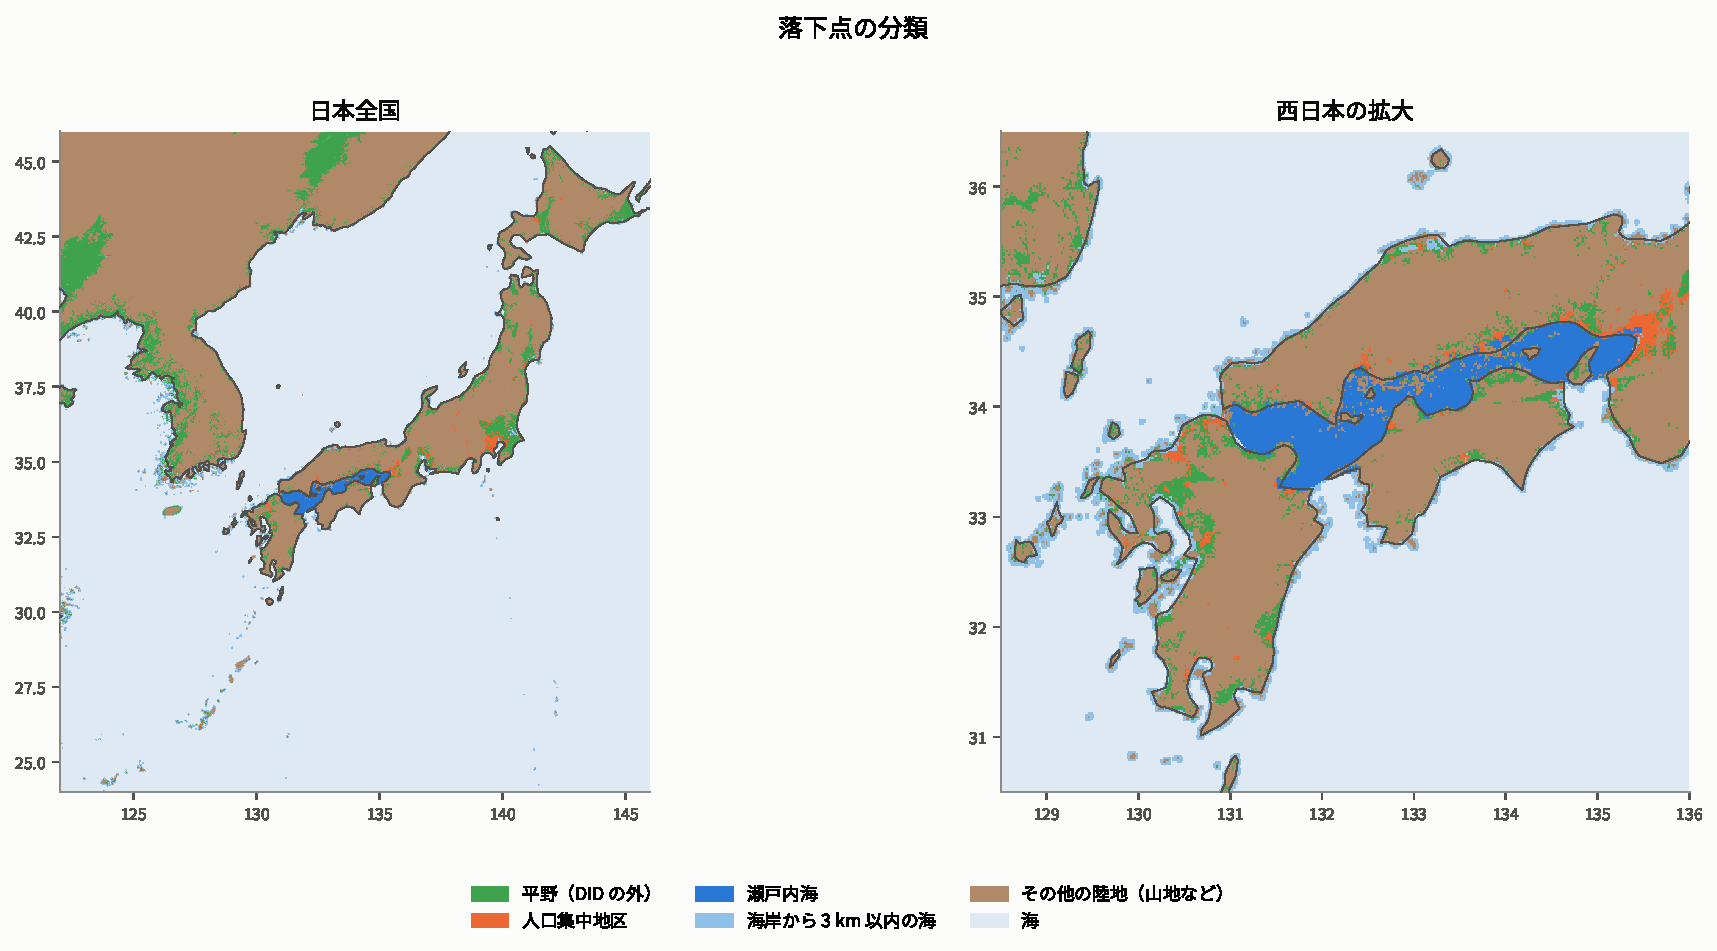
\includegraphics[width=\linewidth]{target_mask.pdf}
\caption{落下の目標。緑が平野（DID の外）、濃い青が瀬戸内海、薄い青が海岸から
\SI{3}{\kilo\metre} 以内の海。赤の人口集中地区と茶の山地は目標に含めない。
右は西日本の拡大。}
\label{fig:target}
\end{figure}

\begin{figure}[htbp]
\centering
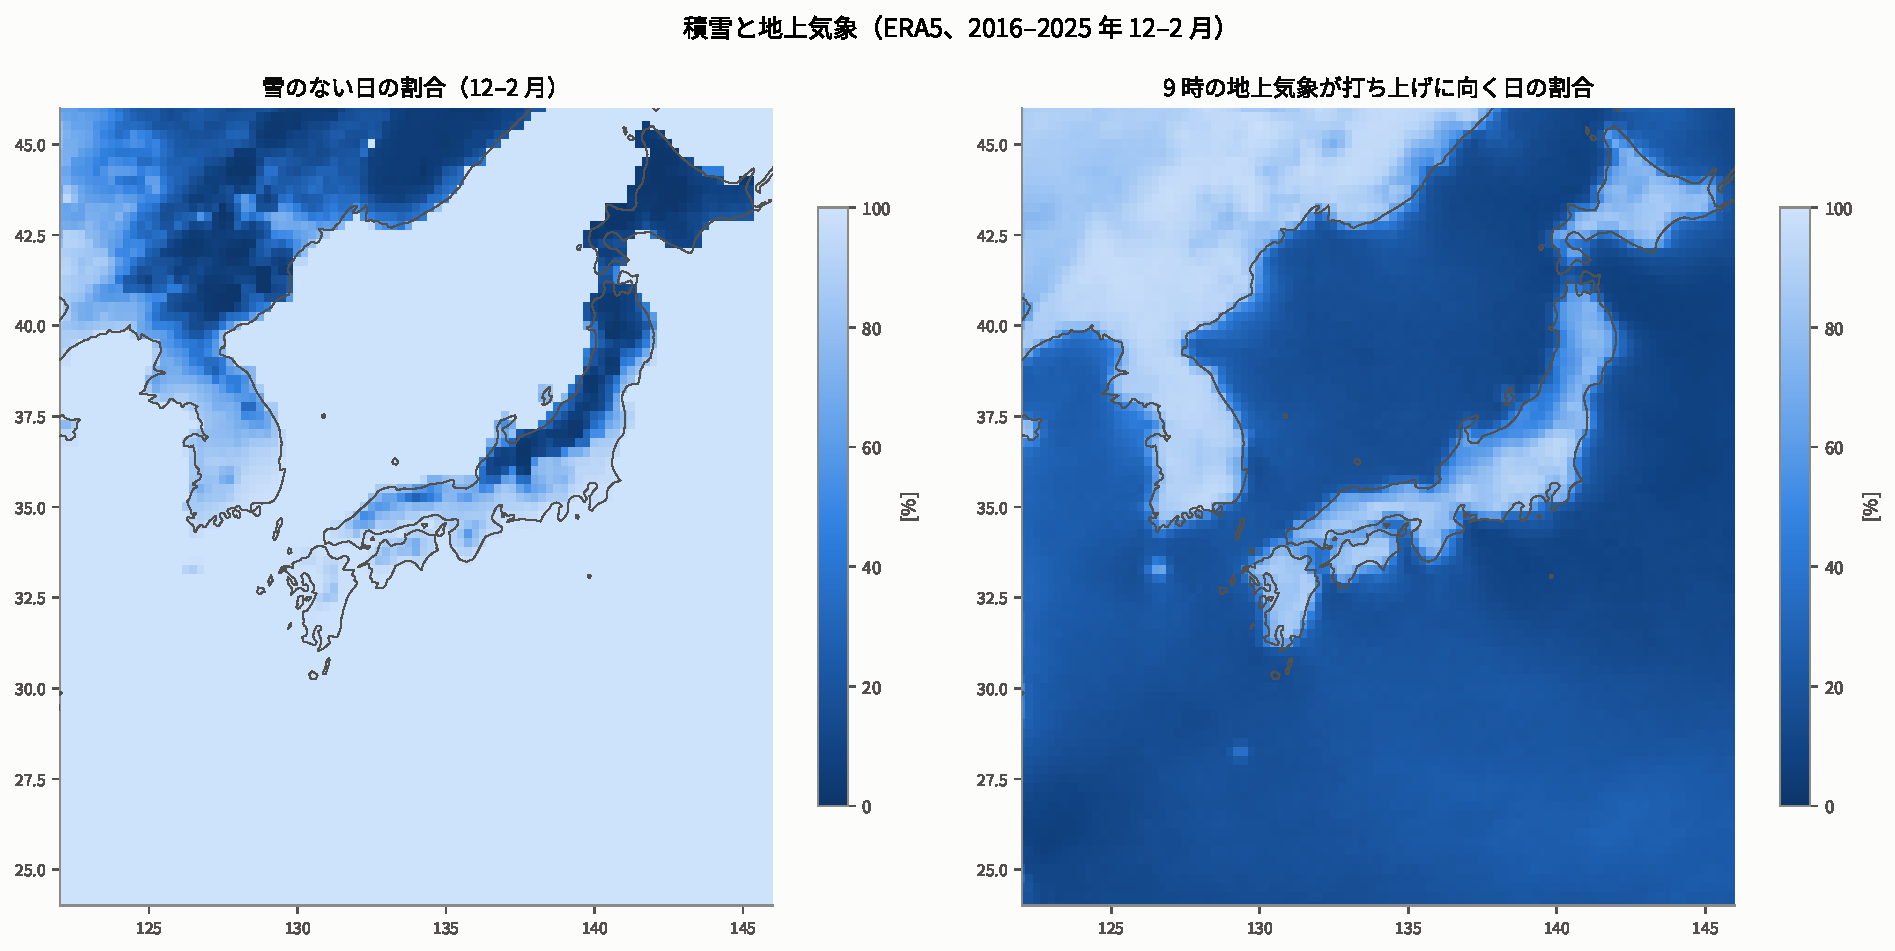
\includegraphics[width=\linewidth]{snow_weather.pdf}
\caption{左: 12--2 月に雪のない日の割合（ERA5、12 時）。右: 9 時の地上気象
（風 \SI{5}{\metre\per\second} 以下・降水 \SI{0.5}{\milli\metre} 未満）が打ち上げに向く日の割合。
日本海側と北日本は雪で、沿岸と島は風で割合が下がる。}
\label{fig:snow}
\end{figure}
